\documentclass[a4paper,10pt]{article}
\usepackage[utf8]{inputenc}
\pdfmapfile{=tengwarscript.map}
\usepackage[T1]{fontenc}
\usepackage{inconsolata}
\usepackage{lmodern}
\usepackage[french]{babel}
\usepackage[squaren, Gray]{SIunits}
\usepackage{circuitikz}
\usepackage{graphicx}
\usepackage{amsmath}
\usepackage{amssymb}
\usepackage{mathrsfs}
\usepackage{subfigure}
\usepackage[absolute]{textpos}
\usepackage{url} 
\usepackage[toc]{appendix}
\usepackage{array}
\usepackage[final]{pdfpages}
\usepackage{listings}
\usepackage[Lenny]{fncychap}
\usepackage{multirow}
\usepackage{ragged2e}
\usepackage{verbatim}
\usepackage[top=1.5cm, bottom=1.5cm, left=1.45cm, right=1.45cm]{geometry}
\usepackage[rightcaption]{sidecap}
\usepackage{systeme}
\usepackage{listings}
\usepackage{courier}
\usepackage{color}
\usepackage{here}
\usepackage[annataritalic]{tengwarscript}
\usepackage{enumitem}
\usepackage{lscape}

%%%%%%%%%%%%%%%%
%						%
%	Listing code Java		%
%						%
%%%%%%%%%%%%%%%%

\definecolor{pblue}{rgb}{0.13,0.13,1}
\definecolor{pgreen}{rgb}{0,0.5,0}
\definecolor{pred}{rgb}{0.9,0,0}

\usepackage{listings}
\lstset{language=Java,
  showspaces=false,
  showtabs=false,
  breaklines=true,
  showstringspaces=false,
  breakatwhitespace=true,
  commentstyle=\color{pgreen},
  keywordstyle=\color{pblue},
  stringstyle=\color{pred},
  basicstyle=\ttfamily,
}


\newcommand{\HRule}{\rule{\linewidth}{0.5mm}}

\begin{document}

\begin{titlepage}

  \begin{center}

% Upper part of the page

    \textsc{\Large Universite Catholique de Louvain}\\[1cm]

    \textsc{\LARGE{Projet : Programming language concepts  }}\\[1cm]


% Title
    \HRule \\[0.35cm]
    {\huge \bfseries Pokemoz}\\
    \HRule \\[0.35cm]
        \end{center}
      \begin{figure}[h!]
      \begin{center}
      
\includegraphics[height=13cm]{pika.png}
      \end{center}
      \end{figure}

    \begin{center}
    \HRule \\[0.2cm]
  \end{center}

    \begin{minipage}{0.48\textwidth}
      \begin{flushleft} \large
        \textit{Auteurs:}\\
        Charles \textsc{Jacquet} (27811200)\\
        Jérôme \textsc{Lemaire} (69601000)\\ \vspace{0.3cm}


      \end{flushleft}
    \end{minipage}
    \begin{minipage}{0.48\textwidth}
      \begin{flushright} \large
        \textit{Cours:} \\
        LINGI1131 \\ \vspace{0.3cm} 
       
        \textit{Titulaire:} \\
        Peter \textsc{Van Roy} \\ \vspace{0.3cm} 
		
		\textit{Assistant:} \\
		Jérémie \textsc{Melchior} \\
      \end{flushright}
    \end{minipage}

    \vfill
% Bottom of the page

    \begin{minipage}{0.3\textwidth}
      \begin{flushleft}
        
\includegraphics[height=2cm]{logo_UCL.jpg}
      \end{flushleft}
    \end{minipage}
    \begin{minipage}{0.3\textwidth}
      \begin{center}
        {\large FSA13BA}\\
        {\large \today}
      \end{center}
    \end{minipage}
    \begin{minipage}{0.3\textwidth}
      \begin{flushright}
        
\includegraphics[height=2cm]{logo_EPL.jpg}
      \end{flushright}
    \end{minipage}
\end{titlepage}

\section*{Introduction}

The game Pokemoz was designed for the class LINGI1131. We have followed the project instructions but also added a little personal touch. 
In order to be closer to the reality, the wild Pokemoz evolve through the game and can acquire experience during combats but also over time.
After a combat, if his Pokemoz is wounded or dead, the head trainer has to go back to his starting point, his house, to cure it or bring it back to life. 

The artificial intelligence provided to our head trainer consists of making his Pokemoz evolve to the tenth level through various fights, while curing it when it’s been hurt or lost a fight. 
Once the tenth level completed, the trainer takes the shortest way to reach the exit.

\section*{Structure of the code and implementation choices}

First, the structure of the three main elements will be presented: the Pokemoz, the trainers and the maps.\\

We have represented the Pokemoz with a record that has the following structure \\
\textbf{Pokemoz = p(type: name:  hp:  lx: xp: )} \\
Where
\begin{itemize}
\item type:  atom that can take 3 different values : grass/fire/water 
\item    name: string representative of the name of the pokemoz
\item    hp: int representative the health status of the pokemoz
\item    lx: int representative the level of the pokemoz
\item    xp: int representative the experience of the pokemoz \\ 

\end{itemize}    


We have represented the trainers with a record that has the following structure \\
\textbf{Trainer = t(p: x:X y:Y handle: type:wild/persoPrincipal name:Name)}\\
Where 
\begin{itemize}
\item   	p: PortObject of the trainer’s pokemoz
\item x: int representative of the abscisse of the position of the trainer on the map 
\item y: int representative of the ordinate of the position of the trainer on the map 
\item handle: graphics components of the trainer 
\item type: atom that can take 2 different values : wild or persoPrincipal
\item name: String representative of the name of the trainer \\
\end{itemize}


Maps are represented as matrices built with a tuple of tuples. The road map’s matrices are filled with zeroes or ones. A value of 1 represents the fact that there is tall grass at that position while a value of 0 means that a road passes through that position.

\paragraph{}
The trainers map contains values of either N or 1000. A value of  N nonzero  represents that a wild trainer N stands on the position, N is the ‘atom’ which represent the wild trainer in the record used to stock them. A value of 1000 means that the head trainer is there and finally a value of 0 represents the fact that the position is free of trainer.

\paragraph{}
In order to design the game, 5 types of PortObject were used. We have included the Pokemoz and the trainers in PortObjects to be able to update them and accede to their information during the events (fights, displacements, treatments …) that they live throughout the game.  

\paragraph{}
We have decided to use three maps. 
The first one is the visual representation of the trainers and their situation: it’s with this map that the player interacts. 
The two others maps are not see by the player, they are used as support for the visual representation: 
\begin{itemize}
\item The first map is used to represent the grass areas on the roads. 
\item The second one virtually represents the position and displacements of the trainers and is included in a PortObject because it is frequently updated and questioned about its state. 
\end{itemize}

\paragraph{}
Finally, the two lasts PortObjects enabling us to stop the displacements of the trainers while a combat is running and to start one combat at a time.  But unfortunately it doesn’t work as well as we’d imagined it. Actually at that time we didn’t know PortObjects with states and we tried to create that with these two PortObjects. But some problems still encounter due to the fact that unlike state, our functions aren’t atomic ones.  That’s (with all what we added to try to counter that), the only reason why some times, more than one combat can happen. Or also those trainers can move a little in some case while a combat is already underway (If the movement had start before the ‘pause’ event or also if more than one combat are started and one stops). When we notice that, we’ve seen that our architecture doesn’t allow use to add state and we had not enough time left to change all our code.
\paragraph{}
We invite you to take a look at the component and state diagrams to understand the interactions between the PortObjects.

      
\begin{figure}[h!]
      \begin{center}
      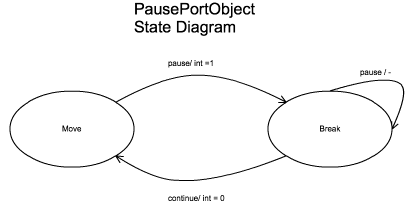
\includegraphics[scale=1]{State_diag_PPO.png}
      \end{center}
      \end{figure}
      
\begin{figure}[h!]
      \begin{center}
      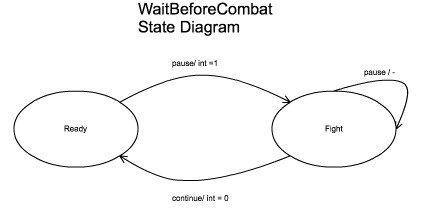
\includegraphics[scale=1]{State_diag_WBC.png}
      \end{center}
      \end{figure}
\begin{landscape}
\begin{figure}[h!]
      \begin{center}
     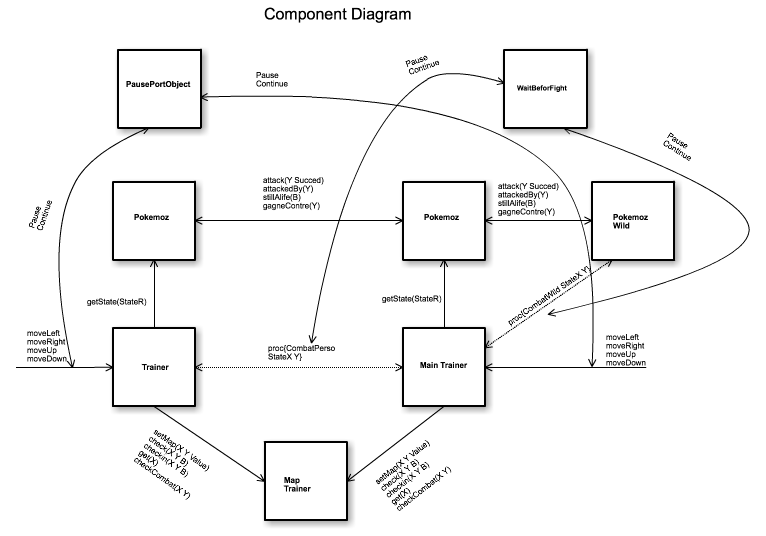
\includegraphics[scale=0.98]{Component_diag.png}
      \end{center}
      \end{figure}
      \end{landscape}

\end{document}